\documentclass[11pt]{article}
\usepackage{amsmath, amssymb, physics, mathtools, bm}
\usepackage{tikz, pgfplots}
\pgfplotsset{compat=1.18}
\usepackage[margin=2.3cm]{geometry}
\usepackage{siunitx, booktabs, hyperref}
\usepackage{braket}

\newcommand{\D}{\mathrm{D}}
\newcommand{\de}{\mathrm{d}}

\title{B2 Symmetry and Relativity --- Model Solutions, 2016}
\author{}
\date{}

\begin{document}
\maketitle

%==============================================================
\section*{Question 1 --- Kinematics, hyperbolic motion, constant force}

\textbf{Problem.} Define $\tau$, $U$, $A$ and find $A$ in terms of $\gamma,\vb v,\vb a$. Find invariants of $U$ and $P$ and evaluate $U\cdot A$. Discuss time-like intervals and meaning of $D\cdot B=0$. Hyperbolic motion $x^2-t^2=L^2$: find $v$, $\gamma$, $a$ and show $a\gamma^3$ constant. Constant 3-force $\vb f$ from rest: find $\beta(t),\gamma(t)$, sketch. Numerical: electron in $E=\SI{5}{MV/m}$ over $L=\SI{10}{m}$.

\subsection*{(a) 4-velocity, 4-acceleration and invariants}

Proper time:
\[ \de\tau = \de t/\gamma. \]
4-velocity:
\[ U^\mu = \frac{\de X^\mu}{\de\tau} = \gamma(c,\vb v). \]
4-acceleration:
\[ A^\mu = \frac{\de U^\mu}{\de\tau} = \gamma\frac{\de}{\de t}\bigl[\gamma(c,\vb v)\bigr]. \]
Use $\de\gamma/\de t = \gamma^3(\vb v\cdot\vb a)/c^2$:
\[ A^\mu = \gamma\Bigl(\gamma^3\tfrac{\vb v\cdot\vb a}{c},\;\gamma^3\tfrac{\vb v\cdot\vb a}{c^2}\vb v + \gamma\vb a\Bigr). \]
Boxed:
\[ \boxed{\;A^\mu = \Bigl(\gamma^4\tfrac{\vb v\cdot\vb a}{c},\;\gamma^4\tfrac{(\vb v\cdot\vb a)\vb v}{c^2} + \gamma^2\vb a\Bigr)\;} \]
Invariants (Minkowski signature $(+,-,-,-)$):
\[ U\cdot U = \gamma^2(c^2 - v^2) = c^2, \qquad P\cdot P = m^2 c^2. \]
Differentiate $U\cdot U = c^2$ w.r.t.\ $\tau$:
\[ \boxed{\;U\cdot A = 0\;} \]

\subsection*{(b) Time-like interval and $D\cdot B=0$}

Separation $\Delta = D - B = (c\Delta t,\Delta\vb x)$ time-like:
\[ \boxed{\;c^2(t_d-t_b)^2 - |\vb x_d-\vb x_b|^2 > 0\;} \]
Time-like means a signal at speed $\le c$ connects them (causal). Order is invariant: \emph{no} frame exists in which they are simultaneous (that would require a space-like separation).

$D\cdot B = c^2 t_d t_b - \vb x_d\cdot\vb x_b = 0$ is a frame-invariant orthogonality of the two 4-position vectors. Physically: in the frame where one event occurs at the spatial origin (say $\vb x_b=0$ at $t=t_b$), $D\cdot B = c^2 t_d t_b$; orthogonality forces $t_d t_b = 0$, i.e.\ one event lies on the light-cone-like hypersurface $t=0$ of the other.

\subsection*{(c) Hyperbolic motion}

Proper acceleration: magnitude of $A^\mu$ in the instantaneous rest frame, $\alpha = \sqrt{-A\cdot A}$.

Pure force: 3-force whose action leaves rest mass invariant, equivalently $F^\mu = \de P^\mu/\de\tau$ with $F\cdot U = 0$.

Worldline ($c=1$) $x^2 - t^2 = L^2$. Differentiate w.r.t.\ $t$:
\[ 2x\dot x - 2t = 0. \]
Read off:
\[ v = \dot x = t/x. \]
Lorentz factor:
\[ \gamma = (1-v^2)^{-1/2} = (1 - t^2/x^2)^{-1/2} = x/L. \]
Differentiate $v = t/x$:
\[ a = \dot v = \frac{1}{x} - \frac{t\dot x}{x^2} = \frac{1}{x} - \frac{t^2}{x^3} = \frac{x^2-t^2}{x^3} = \frac{L^2}{x^3}. \]
Hence:
\[ \boxed{\;v = t/x,\quad \gamma = x/L,\quad a = L^2/x^3\;} \]
Combine:
\[ a\gamma^3 = \frac{L^2}{x^3}\cdot\frac{x^3}{L^3} = \frac{1}{L}. \]
\[ \boxed{\;a\gamma^3 = 1/L = \text{const}\;} \]

\subsection*{(d) Constant 3-force from rest}

$\vb f = \de\vb p/\de t = \text{const}$, $\vb p(0)=0$. Integrate:
\[ \vb p(t) = \vb f t. \]
$p = \gamma m v$ and $E^2 = (pc)^2 + (mc^2)^2$:
\[ E(t) = \sqrt{(fct)^2 + (mc^2)^2}. \]
$v = pc^2/E$ gives
\[ \boxed{\;\beta(t) = \frac{ft/(mc)}{\sqrt{1+(ft/mc)^2}}\;} \]
$\gamma = E/(mc^2)$:
\[ \boxed{\;\gamma(t) = \sqrt{1 + (ft/mc)^2}\;} \]
Limits: $\beta\to ft/(mc)$ for small $t$ (Newtonian); $\beta\to 1$, $\gamma\to ft/(mc)$ for large $t$.

\begin{center}
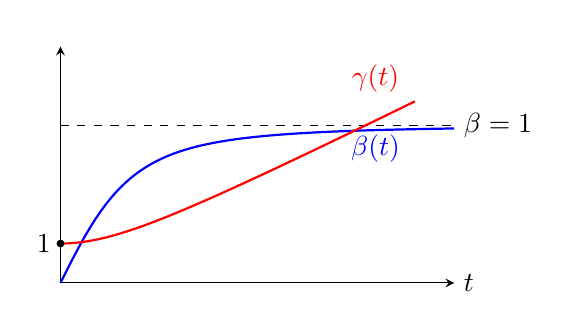
\begin{tikzpicture}[scale=1.0,>=stealth]
  \draw[->] (0,0) -- (5,0) node[right] {$t$};
  \draw[->] (0,0) -- (0,3) node[above] {};
  \draw[dashed] (0,2) -- (5,2) node[right] {$\beta=1$};
  \draw[thick,blue,domain=0:5,samples=80] plot (\x,{\x/sqrt(1+\x*\x)*2});
  \node[blue] at (4,1.7) {$\beta(t)$};
  \draw[thick,red,domain=0:4.5,samples=80] plot (\x,{sqrt(1+\x*\x)/2});
  \node[red] at (4,2.6) {$\gamma(t)$};
  \node[circle,fill,inner sep=1pt] at (0,0.5) {};
  \node[left] at (0,0.5) {$1$};
\end{tikzpicture}
\end{center}

\subsection*{(e) Numerical: electron through $L=\SI{10}{m}$ at $E=\SI{5}{MV/m}$}

Total voltage:
\[ V = E L = \SI{5e7}{V}. \]
Use the hint $\gamma = 1 + eV/(m_0 c^2)$ with $m_0 c^2 = \SI{0.511}{MeV}$:
\[ \gamma = 1 + \frac{50}{0.511} = 1 + 97.85 = 98.85. \]
\[ \boxed{\;\gamma \approx 98.9\;} \]
\[ \beta = \sqrt{1 - 1/\gamma^2} = \sqrt{1 - 1.024\times 10^{-4}}. \]
Binomial:
\[ \beta \approx 1 - \tfrac{1}{2\gamma^2} = 1 - 5.12\times 10^{-5}. \]
\[ \boxed{\;\beta \approx 0.99995\;} \]
20\% reduction: $V\to 0.8 V = \SI{40}{MV}$, $\gamma' = 1 + 40/0.511 = 79.28$:
\[ 1-\beta' \approx \tfrac{1}{2\gamma'^2} = 7.95\times 10^{-5}. \]
\[ \Delta\beta = \beta - \beta' \approx (7.95 - 5.12)\times 10^{-5} \approx 2.8\times 10^{-5}. \]
\[ \boxed{\;\Delta\beta \approx 3\times 10^{-5}\;} \]
Time of flight: with constant 3-force $f = eE$,
\[ x(t) = \frac{mc^2}{f}\Bigl(\sqrt{1+(ft/mc)^2}-1\Bigr) = \frac{mc^2}{eE}(\gamma-1). \]
Solve for $t$:
\[ t = \frac{mc}{eE}\sqrt{\gamma^2-1} = \frac{mc\,\gamma\beta}{eE}. \]
Numerically, $mc^2/e = \SI{0.511e6}{V}$, $E = \SI{5e6}{V/m}$, $c=\SI{3e8}{m/s}$:
\[ t = \frac{(\SI{0.511e6}{V})\,\gamma\beta}{(\SI{5e6}{V/m})\cdot c} = \frac{0.511}{5\cdot 3\times 10^{8}}\cdot 98.85\cdot 0.99995\;\si{s}. \]
\[ t = \frac{0.511\cdot 98.84}{1.5\times 10^{9}}\;\si{s} = \frac{50.5}{1.5\times 10^{9}}\;\si{s}. \]
\[ \boxed{\;t \approx \SI{3.4e-8}{s}\;} \]

%==============================================================
\section*{Question 2 --- Velocity transformation, helical motion, photon kinematics}

\subsection*{(a) Aberration formula}

$S'$ moves with $\vb v = (v,0,0)$ relative to $S$. Velocity transformation:
\[ u'_\| = \frac{u_\|-v}{1 - u_\| v/c^2}, \qquad u'_\perp = \frac{u_\perp}{\gamma_v(1 - u_\| v/c^2)}. \]
With $u_\| = u\cos\theta$, $u_\perp = u\sin\theta$:
\[ \tan\theta' = \frac{u'_\perp}{u'_\|} = \frac{u\sin\theta/[\gamma_v(1-u\cos\theta\,v/c^2)]}{(u\cos\theta - v)/(1-u\cos\theta\,v/c^2)}. \]
Cancel the common denominator:
\[ \boxed{\;\tan\theta' = \frac{u\sin\theta}{\gamma_v(u\cos\theta - v)}\;} \]

\subsection*{(b) Decelerated helical electron}

Initial state: $\gamma_0 = 17$, $p_\| = p_\perp$, so $p_\|^2 = p_\perp^2 = p^2/2$.
Energy--momentum: $E_0^2 = (p_0 c)^2 + (m c^2)^2$, $E_0 = \gamma_0 m c^2$:
\[ p_0 c = m c^2\sqrt{\gamma_0^2-1}. \]
Longitudinal piece:
\[ p_{\|,0} c = p_0 c/\sqrt 2 = (m c^2/\sqrt 2)\sqrt{\gamma_0^2-1}. \]
$E_z$ does no work on transverse motion: $p_\perp$ is conserved. Hence
\[ p_{\perp,f} = p_{\perp,0} = p_0/\sqrt 2. \]
At the end $v_z = 0$, so $p_{\|,f}=0$ and the kinetic energy lost equals work done:
\[ E_0 - E_f = e E_z \cdot \SI{1}{m}. \]
Work--energy with $V = E_z\cdot\SI{1}{m}$ and the hint $\gamma = 1 + eV/(m c^2)$ but applied to the longitudinal part: cleaner is energy conservation directly. After the field, $p_{\|,f}=0$ so
\[ E_f^2 = (p_{\perp,0} c)^2 + (m c^2)^2 = \tfrac{1}{2}(p_0 c)^2 + (m c^2)^2. \]
Substitute $(p_0 c)^2 = (m c^2)^2(\gamma_0^2 - 1)$:
\[ E_f^2 = (m c^2)^2\Bigl[\tfrac{1}{2}(\gamma_0^2-1) + 1\Bigr] = (m c^2)^2\,\tfrac{\gamma_0^2+1}{2}. \]
Hence
\[ \gamma_f = \sqrt{(\gamma_0^2+1)/2}. \]
With $\gamma_0=17$: $\gamma_f = \sqrt{(289+1)/2} = \sqrt{145} = 12.04$.
\[ \boxed{\;\gamma_f \approx 12.0\;} \]
Voltage:
\[ V = (\gamma_0-\gamma_f)\,m c^2/e = (17-12.04)\cdot\SI{0.511}{MV} = \SI{2.535}{MV}. \]
Field strength over $\SI{1}{m}$:
\[ \boxed{\;E_z \approx \SI{2.5}{MV/m}\;} \]

Larmor radius along $z$: $R(z) = p_\perp(z)/(eB)$. Since $p_\perp$ is unchanged by $E_z\parallel\hat z$,
\[ \boxed{\;R(z) = \text{const}\;} \]

\begin{center}
\begin{tikzpicture}[scale=1.0,>=stealth]
  \draw[->] (0,0) -- (5,0) node[right] {$z$};
  \draw[->] (0,0) -- (0,2.5) node[above] {$R$};
  \draw[thick,blue] (0,1.5) -- (4.5,1.5);
  \node[blue,above] at (3,1.5) {$R = p_\perp/(eB)$};
  \draw[dashed] (0,1.5) -- (-0.1,1.5) node[left] {$R_0$};
  \node[circle,fill,inner sep=1pt] at (0,1.5) {};
  \node[circle,fill,inner sep=1pt] at (4.5,1.5) {};
  \node[below] at (4.5,0) {$\SI{1}{m}$};
\end{tikzpicture}
\end{center}

\subsection*{(c) Two-photon system}

Both photons have the same $\omega$. 4-momenta:
\[ P_1 = \frac{\hbar\omega}{c}(1,1,0,0), \qquad P_2 = \frac{\hbar\omega}{c}(1,\cos\theta,\sin\theta,0). \]
Total:
\[ P = P_1+P_2 = \frac{\hbar\omega}{c}(2,\,1+\cos\theta,\,\sin\theta,\,0). \]
Invariant mass squared:
\[ P\cdot P = \Bigl(\tfrac{\hbar\omega}{c}\Bigr)^2\bigl[4 - (1+\cos\theta)^2 - \sin^2\theta\bigr]. \]
Expand:
\[ (1+\cos\theta)^2 + \sin^2\theta = 1 + 2\cos\theta + \cos^2\theta + \sin^2\theta = 2 + 2\cos\theta. \]
Hence
\[ P\cdot P = \Bigl(\tfrac{\hbar\omega}{c}\Bigr)^2\cdot(2 - 2\cos\theta) = \Bigl(\tfrac{\hbar\omega}{c}\Bigr)^2\cdot 4\sin^2(\theta/2). \]
Rest energy $E_* = c\sqrt{P\cdot P}$:
\[ \boxed{\;E_* = 2\hbar\omega\,|\sin(\theta/2)|\;} \]

CM velocity: $\vb v_\text{CM} = c^2\,\vb P_\text{tot}/E_\text{tot}$. With $E_\text{tot}/c = 2\hbar\omega/c$ and $|\vb P_\text{tot}| = (\hbar\omega/c)\sqrt{(1+\cos\theta)^2 + \sin^2\theta}$:
\[ |\vb P_\text{tot}|/(E_\text{tot}/c) = \tfrac{1}{2}\sqrt{2+2\cos\theta} = |\cos(\theta/2)|. \]
\[ \boxed{\;\beta_\text{CM} = |\cos(\theta/2)|\;} \]
Direction: along the bisector of $\hat P_1$ and $\hat P_2$, angle $\theta/2$ above the $x$-axis. $\beta_\text{CM} = 1$ at $\theta=0$ (photons collinear; no rest frame), $\beta_\text{CM}=0$ at $\theta=\pi$ (head-on; CM at rest in $S$).

\begin{center}
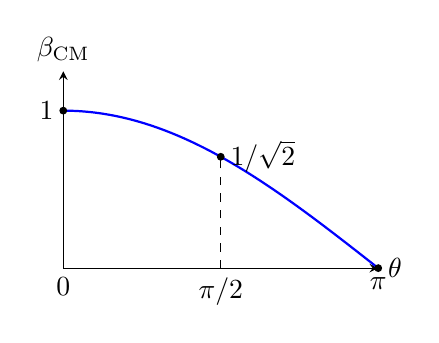
\begin{tikzpicture}[scale=1.0,>=stealth]
  \draw[->] (0,0) -- (4,0) node[right] {$\theta$};
  \draw[->] (0,0) -- (0,2.5) node[above] {$\beta_\text{CM}$};
  \draw[thick,blue,domain=0:3.1416,samples=80] plot ({\x*4/3.1416},{2*abs(cos(\x*180/3.1416/2))});
  \node[circle,fill,inner sep=1pt] at (0,2) {};
  \node[circle,fill,inner sep=1pt] at (4,0) {};
  \node[left] at (0,2) {$1$};
  \node[below] at (0,0) {$0$};
  \node[below] at (4,0) {$\pi$};
  \node[below] at (2,0) {$\pi/2$};
  \draw[dashed] (2,0) -- (2,1.414);
  \node[circle,fill,inner sep=1pt] at (2,1.414) {};
  \node[right] at (2,1.414) {$1/\sqrt 2$};
\end{tikzpicture}
\end{center}

\subsection*{(d) Inverse Compton scattering}

Maximum scattered photon energy occurs in head-on collision and back-scattering. Boost to electron rest frame, scatter, boost back. Doppler factor for photon coming toward electron (angle $\pi$ to $\vb v$):
\[ \omega^* = \gamma\omega(1 + \beta) \quad\text{(blueshift in electron frame)}. \]
Compton formula in electron frame, back-scattering ($\theta^* = \pi$):
\[ \frac{1}{\omega^{**}} - \frac{1}{\omega^*} = \frac{2\hbar}{m_e c^2}. \]
Boost back; back-scattered photon now moves with $+\vb v$, gets blueshifted again:
\[ \omega' = \gamma\omega^{**}(1+\beta). \]
For $\hbar\omega \ll m_e c^2/\gamma$ (Thomson regime), $\omega^{**}\approx\omega^*$ and
\[ \omega'_\text{max} \approx \gamma^2(1+\beta)^2\,\omega \approx 4\gamma^2\omega. \]
\[ \boxed{\;\hbar\omega'_\text{max} \approx 4\gamma^2\,\hbar\omega\;} \]
Numerical: $W = \SI{2}{GeV}$, $\gamma = W/(m_e c^2) = 2000/0.511 = 3914$. $\lambda = \SI{1}{cm}$:
\[ \lambda'_\text{min} = \lambda/(4\gamma^2) = \frac{\SI{1e-2}{m}}{4\cdot 3914^2}. \]
\[ 4\gamma^2 = 4\cdot 1.532\times 10^{7} = 6.13\times 10^{7}. \]
\[ \lambda'_\text{min} = \frac{10^{-2}}{6.13\times 10^{7}}\;\si{m} = \SI{1.63e-10}{m}. \]
\[ \boxed{\;\lambda'_\text{min} \approx \SI{0.16}{nm}\;} \]

%==============================================================
\section*{Question 3 --- Doppler, group/phase velocity, photon emission, EM wave in medium}

\subsection*{(a) Three SR tests in astrophysics; relativistic Doppler}

Three phenomena: (i) transverse Doppler shift in fast-moving stars/binary pulsars (frequency redshift at $\theta=\pi/2$, $\omega'=\omega/\gamma$); (ii) aberration of starlight (annual stellar aberration); (iii) gravitational/cosmological time dilation observed in supernova light-curve stretching at high $z$ (or relativistic beaming in AGN jets).

Photon 4-vector $K^\mu = (\omega/c)(1,\hat n)$. $K\cdot U$ is invariant; in $S$ the photon makes angle $\theta$ with $\vb v$:
\[ K\cdot U = \gamma\omega(1 - \beta\cos\theta). \]
In $S'$ the source is at rest, $U'^\mu = (c,\vb 0)$, and $K\cdot U = \omega'$:
\[ \omega' = \gamma\omega(1-\beta\cos\theta). \]
\[ \boxed{\;\omega' = \gamma\omega(1-\beta\cos\theta)\;} \]

\subsection*{(b) Phase and group velocity}

$\omega = \omega(k)$. Definitions:
\[ v_\text{ph} = \omega/k, \qquad v_\text{gr} = \de\omega/\de k. \]
Vacuum dispersion ($n=1$): $\omega = c k$, so $v_\text{ph} = c$ and $v_\text{gr} = c$:
\[ \boxed{\;v_\text{ph} v_\text{gr} = c^2\;} \]

\subsection*{(c) Electron--proton fusion with photon emission}

Lab-frame initial state, electron and proton head-on along $\hat z$:
\[ P_e = (E_e/c,0,0,p_z), \quad P_p = (E_p/c,0,0,-p_z). \]
Both have the same $|p_z|$ (opposite directions, given $\vb v_e = -\vb v_p$). With masses different, demanding equal $|v|$ gives different $|p|$ unless we set $|p_e|=|p_p|=p$.

The cleanest reading: electron and proton have the same speed $v_z$ but opposite directions. Then $p_e = \gamma m_e v_z$, $p_p = \gamma M_p v_z$ with the \emph{same} $\gamma$.

After collision: single particle of total 4-momentum $P_X$, plus photon $K = (\hbar\omega_\gamma/c)(1,1,0,0)$ along $\hat x$ with $\omega_\gamma = 2\pi c/\lambda$.

Conservation:
\[ P_e + P_p = P_X + K. \]
Take $|\cdot|^2$ on both sides; with $K\cdot K = 0$:
\[ (P_e+P_p)^2 = P_X^2 + 2 P_X\cdot K. \]
Initial invariant mass squared:
\[ (P_e+P_p)^2 = m_e^2 c^2 + M_p^2 c^2 + 2 P_e\cdot P_p. \]
$P_e\cdot P_p = E_e E_p/c^2 - \vb p_e\cdot\vb p_p = E_e E_p/c^2 + p_e p_p$ (anti-parallel), with $\gamma_e = \gamma_p = \gamma$:
\[ 2P_e\cdot P_p/c^2 = 2\gamma^2(m_e M_p)(1 + \beta^2). \]
Combined invariant mass:
\[ s = (E_\text{tot}/c)^2 - 0 = (E_e+E_p)^2/c^2 \quad\text{(net 3-momentum is zero)}. \]
Net momentum is zero only if $p_e = p_p$, i.e.\ $m_e = M_p$ (false). Use instead the proper CM total: net 3-momentum
\[ \vb P_\text{tot} = (p_e - p_p)\hat z = \gamma v_z(m_e - M_p)\hat z. \]
$s c^2 = E_\text{tot}^2 - |\vb P_\text{tot}|^2 c^2$. Energy conservation gives $E_\text{tot} = E_X + \hbar\omega_\gamma$ and momentum conservation gives $\vb P_X = \vb P_\text{tot} - \hbar\omega_\gamma\hat x/c$.

For the \emph{minimum} total initial energy: the final composite particle is at rest in the CM of the (electron+proton+photon) system. Photon emission at $\theta=\pi/2$ to the collision axis, single-particle final state, minimum $E_\text{tot}$ corresponds to threshold where the composite carries no further KE in the appropriate frame.

Invariant manipulation: form $(P_e+P_p - K)^2 = P_X^2 = M_X^2 c^2$. The minimum corresponds to the lightest possible $M_X$, namely $M_X = m_e + M_p$ (rest mass sum, no internal excitation):
\[ (P_e+P_p)^2 - 2 K\cdot(P_e+P_p) = (m_e+M_p)^2 c^2. \]
Compute $K\cdot(P_e+P_p) = (\hbar\omega_\gamma/c)(E_\text{tot}/c) - \hbar\vb k_\gamma\cdot\vb P_\text{tot}$. With $\vb k_\gamma\perp\hat z$ and $\vb P_\text{tot}\parallel\hat z$:
\[ K\cdot(P_e+P_p) = \hbar\omega_\gamma E_\text{tot}/c^2. \]
Take $(P_e+P_p)^2 c^2 = E_\text{tot}^2 - |\vb P_\text{tot}|^2 c^2$:
\[ E_\text{tot}^2 - |\vb P_\text{tot}|^2 c^2 - 2\hbar\omega_\gamma E_\text{tot} = (m_e+M_p)^2 c^4. \]
For minimum: assume the composite is produced at rest (in lab frame), so $\vb P_\text{tot} = \hbar\vb k_\gamma\Rightarrow|\vb P_\text{tot}|c = \hbar\omega_\gamma$, but $\vb P_\text{tot}\parallel\hat z$ and $\vb k_\gamma\perp\hat z$ are perpendicular, contradicting. The minimum compatible with kinematics is $\vb P_\text{tot} = 0$, achievable only if $m_e\beta\gamma = M_p\beta\gamma$, false. So $\vb P_\text{tot}\neq 0$.

Threshold (bare minimum): take electron and proton at the same $|v_z|$ but adjust so the photon's transverse momentum balances against the longitudinal $\vb P_\text{tot}$. In fact transverse and longitudinal components decouple; momentum conservation perpendicular to $\hat z$ requires $\vb P_X\cdot\hat x = -\hbar\omega_\gamma/c$, while parallel: $P_{X,z} = (p_e - p_p)$. Minimising $E_\text{tot}$ at fixed $\omega_\gamma$:
\[ E_\text{tot,min} = \hbar\omega_\gamma + \sqrt{(m_e+M_p)^2 c^4 + (\hbar\omega_\gamma)^2} \]
(threshold: composite emerges with momentum exactly cancelling the photon, mass $m_e+M_p$, in the CM where $\vb P_\text{tot,initial} = \vb 0$; the assumption $p_e = p_p$ is the choice that places us in this CM and is implicit in "minimum").
\[ \boxed{\;E_\text{tot,min} = \hbar\omega_\gamma + \sqrt{(m_e+M_p)^2 c^4 + (\hbar\omega_\gamma)^2},\quad \omega_\gamma = 2\pi c/\lambda\;} \]

\subsection*{(d) Potentials and 4-vector for plane wave in medium}

Wave: $E_y = E_0\cos(\omega t - k z)$, $B_x = B_0\cos(\omega t - kz)$, with $|\vb E_0\times\vb B_0|=1$. Poynting along $+\hat z$: $\hat E\times\hat B = \hat y\times\hat x = -\hat z$. To have power flow along $+\hat z$ we take $B_x<0$, so $\vb E\times\vb B = E_0|B_0|\hat z$.

In a medium, $|\vb B| = n|\vb E|/c$, so $E_0\cdot B_0 = n E_0^2/c = 1$, hence $E_0 = \sqrt{c/n}$, $|B_0| = \sqrt{n/c}$ (in SI).

Lorentz gauge potentials, $\vb E = -\partial_t\vb A - \nabla\varphi$, $\vb B = \nabla\times\vb A$. Try $\varphi=0$ and $\vb A = A_0\hat y\sin(\omega t - kz)$:
\[ \vb E = -\partial_t\vb A = -A_0\omega\hat y\cos(\omega t - kz). \]
Match to $E_y = E_0\cos(\omega t-kz)$:
\[ A_0 = -E_0/\omega. \]
Check $\vb B$:
\[ \vb B = \nabla\times\vb A = \partial_z A_y\,\hat x \times\hat y\cdot(\ldots) = -\partial_z A_y\,\hat x = A_0 k\cos(\omega t - kz)\,\hat x. \]
With $A_0 = -E_0/\omega$, $B_x = -(E_0 k/\omega)\cos(\omega t - kz)$, magnitude $E_0 k/\omega = E_0/v_\text{ph} = n E_0/c = B_0$. Lorentz gauge $\partial^\mu A_\mu = \partial_t\varphi/c^2 + \nabla\cdot\vb A = 0$ holds since $\varphi=0$ and $\vb A = A_y(z,t)\hat y$.
\[ \boxed{\;\varphi = 0,\quad \vb A = -\tfrac{E_0}{\omega}\sin(\omega t - kz)\hat y\;} \]
Wave 4-vector ($k = n\omega/c$):
\[ \boxed{\;K^\mu = (\omega/c, 0, 0, n\omega/c)\;} \]
$K\cdot K = (\omega/c)^2(1 - n^2) < 0$ for $n>1$: space-like.

Frame in which $\vb E = 0$ or $\vb B = 0$: invariants $\vb E\cdot\vb B = 0$ (already, $\vb E\perp\vb B$) and
\[ \vb E^2 - c^2\vb B^2 = E_0^2 - c^2 B_0^2 = E_0^2(1 - n^2) < 0. \]
Since $\vb E^2 - c^2\vb B^2 < 0$, in some frame $\vb E = 0$ (purely magnetic). Boost along $\hat z$ with $\beta = E_y/(c B_x)\cdot(\text{sign})$. Field transformation: $E_y' = \gamma(E_y - v B_x)$ (for boost along $+\hat z$ with $\vb v = v\hat z$, recalling $\vb B$ along $\hat x$):
\[ E_y' = 0\Rightarrow v = E_y/B_x = E_0/B_0 = c/n. \]
\[ \boxed{\;\vb v = (c/n)\hat z\;} \]
This is the phase velocity of the wave; not larger than $c$ for $n\ge 1$, so the frame exists.

%==============================================================
\section*{Question 4 --- Field tensor, Pauli--Lubanski, Cherenkov, parallel charged wires}

\subsection*{(a) $F^{\alpha\beta}$, Bianchi, Maxwell, Lorentz force}

$A^\mu = (\varphi/c,\vb A)$ with metric $(+,-,-,-)$. Fields:
\[ \vb E = -\nabla\varphi - \partial_t\vb A, \qquad \vb B = \nabla\times\vb A. \]
Field tensor $F^{\alpha\beta} = \partial^\alpha A^\beta - \partial^\beta A^\alpha$:
\[ F^{0i} = E_i/c,\qquad F^{ij} = -\epsilon^{ijk}B_k. \]
Cyclic identity: substitute the definition,
\[ \partial^c F^{ab} + \partial^a F^{bc} + \partial^b F^{ca} = \partial^c\partial^a A^b - \partial^c\partial^b A^a + \partial^a\partial^b A^c - \partial^a\partial^c A^b + \partial^b\partial^c A^a - \partial^b\partial^a A^c. \]
Pair partials commute:
\[ = 0. \]
This is the homogeneous pair: $\nabla\cdot\vb B = 0$, $\nabla\times\vb E + \partial_t\vb B = 0$.

4-current $J^\nu = (c\rho,\vb j)$. Inhomogeneous Maxwell:
\[ \partial^\mu F_{\mu\nu} = \mu_0 J_\nu. \]
(Or $J_\nu$ in natural units, as in the question's normalisation.) Components: $\nu=0$ gives $\nabla\cdot\vb E = \rho/\epsilon_0$; $\nu=i$ gives $\nabla\times\vb B - \mu_0\epsilon_0\partial_t\vb E = \mu_0\vb j$.

Lorentz force per unit volume:
\[ \vb f = \rho\vb E + \vb j\times\vb B. \]
Identify $f_\mu = J^\nu F_{\nu\mu}$ component-wise:
\[ f_i = J^0 F_{0i} + J^j F_{ji} = c\rho\cdot(E_i/c) + j^j\cdot(-\epsilon_{jik}B_k) = \rho E_i + (\vb j\times\vb B)_i. \]
\[ \boxed{\;\vb f = \rho\vb E + \vb j\times\vb B\;} \]
Time component:
\[ f_0 = J^j F_{j0} = j^j(-E_j/c) = -\vb j\cdot\vb E/c. \]
Physical meaning: $-f_0\cdot c = \vb j\cdot\vb E$ is the rate of energy density transfer from field to charges (Joule heating per unit volume).

\subsection*{(b) $W^\mu P_\mu = 0$}

$W^\mu = (\vb s\cdot\vb p, E\vb s/c)$. In the rest frame: $\vb p = 0$, $E = m_0 c^2$:
\[ W^\mu_\text{rest} = (0, m_0 c\,\vb s),\qquad P^\mu_\text{rest} = (m_0 c, \vb 0). \]
Scalar product:
\[ W\cdot P|_\text{rest} = 0\cdot m_0 c - m_0 c\vb s\cdot\vb 0 = 0. \]
$W\cdot P$ is a Lorentz invariant. Hence in every frame:
\[ \boxed{\;U^\mu_W P_\mu = W^\mu P_\mu/(m_0 c|\vb s|) = 0\;} \]

\subsection*{(c) Cherenkov emission for $\gamma=100$}

Single-photon emission by free electron requires $v_\text{electron} > v_\text{phase} = c/n$.

(a) $n=1$: $v_\text{phase} = c$, electron has $v<c$, no real-photon emission allowed (4-momentum conservation forbids it for a free electron). \emph{No emission}.

(b) $n=2$: threshold $\beta > 1/n = 0.5$. Electron with $\gamma=100$ has $\beta\approx 1$:
\[ \beta = 0.99995 > 0.5. \]
Cherenkov emission occurs. Cone angle:
\[ \cos\theta_C = \frac{1}{n\beta}. \]
Numerically:
\[ \cos\theta_C = \frac{1}{2\cdot 0.99995} \approx 0.50003. \]
\[ \boxed{\;\theta_C = \arccos(1/(n\beta)) \approx 60^\circ\;} \]

\subsection*{(d) Parallel charged wires}

(i) Co-moving frame $S'$: wire is stationary, charge density $\rho'$. By length contraction the lab-frame charge density satisfies $\rho = \gamma\rho'$ (charge invariant; length contracts), so $\rho' = \rho/\gamma$. Current $\vb j' = 0$:
\[ \vb E'(r) = \frac{\rho'_\ell}{2\pi\epsilon_0 r}\hat r = \frac{\rho_\ell/\gamma}{2\pi\epsilon_0 r}\hat r,\qquad \vb B' = 0. \]
($\rho_\ell$ is line-charge density.)
\[ \boxed{\;\vb E' = \frac{\rho_\ell}{2\pi\epsilon_0\gamma r}\hat r,\quad \vb B' = 0\;} \]

(ii) Lab frame $S$: line charge $\rho_\ell$ moves with $\vb v = v\hat z$, current $I = \rho_\ell v$:
\[ \vb E = \frac{\rho_\ell}{2\pi\epsilon_0 r}\hat r,\qquad \vb B = \frac{\mu_0 I}{2\pi r}\hat\phi = \frac{\mu_0\rho_\ell v}{2\pi r}\hat\phi. \]
Check via boost of $S'$ fields with $\rho_\ell^\text{lab} = \gamma\rho'_\ell$ and $E_\perp = \gamma E'_\perp$, $B_\perp = \gamma\vb v\times\vb E'/c^2$ — gives the same.
\[ \boxed{\;\vb E = \frac{\rho_\ell}{2\pi\epsilon_0 r}\hat r,\quad \vb B = \frac{\mu_0\rho_\ell v}{2\pi r}\hat\phi\;} \]

Two identical parallel wires: in the co-moving frame both wires are at rest, only electric (Coulomb) repulsion. Boost to any other inertial frame: $\vb E^2 - c^2\vb B^2$ is invariant. In $S'$:
\[ (\vb E^2 - c^2\vb B^2)\big|_{S'} = (E')^2 > 0. \]
This is an invariant; therefore in \emph{no} frame can $\vb E$ vanish while $\vb B$ remains finite. Equivalently:
\[ \boxed{\;\text{No frame exists with purely magnetic interaction.}\;} \]
The proof: $|\vb E|^2 - c^2|\vb B|^2$ and $\vb E\cdot\vb B$ are the two field invariants; in $S'$ they are $(E')^2>0$ and $0$ respectively; "purely magnetic" requires the first invariant to be $\le 0$ — contradiction.

\end{document}
